\tikzstyle{txt} = [text centered, inner sep=0pt]

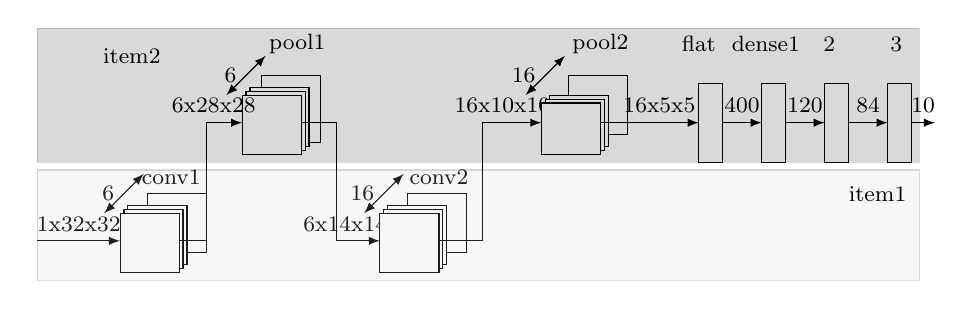
\begin{tikzpicture}[scale=1.0,
z={({0.3cm*cos(45)},{0.3cm*sin(45)})},
>=latex, 
font=\footnotesize,
]

% Big Input images



%CONV1
\draw[fill=white] (0.25+7*0.05,7*0.05) rectangle (1+7*0.05,.75+7*0.05);
\foreach \foreach \z in {2,...,0}  {%
 \draw[fill=white] (0.25+\z*0.05,.1+\z*0.05) rectangle (1+\z*0.05,.85+\z*0.05);
}
\draw (0.9,1.3)node[txt] (conv1){conv1};
\draw[->] (-.8,0.5) -- node[above] {$1$x$32$x$32$} (0.25,0.5);
\draw[<->] (.25-0.2,.85+0*0.05) -- node[left] {$6$} (.25+0.3,.85+0.5);

%MAXPOOL1
\draw[fill=white] (2.5+5*0.05-.7,5*0.05+1.5) rectangle (3.25+5*0.05-.7,0.85+5*0.05+1.5);
\foreach \foreach \z in {2,...,0}  {%
 \draw[fill=white] (2.5+\z*0.05-.7,0.1+\z*0.05+1.5) rectangle (3.25+\z*0.05-.7,.85+\z*0.05+1.5);
}
\draw (3.2-.7,1.5+1.5)node[txt] (conv1){pool1};
\draw[->] (1,0.5) --(1.75-.4,0.5) |- node[above,pos=0.6] {$6$x$28$x$28$} (2.5-.7,0.5+1.5);
\draw[<->] (2.5-0.2-.7,0.85+0*0.05+1.5) -- node[left] {$6$} (2.5+0.3-.7,0.85+0.5+1.5);

%CONV2
\draw[fill=white] (4.75+7*0.05-1.2,7*0.05) rectangle (5.5+7*0.05-1.2,0.75+7*0.05);
\draw (5.5-1.2,1.3)node[txt] (conv1){conv2};
\draw[->] (3.25-.7,0.5+1.5) -- (4-1,0.5+1.5) |- node[above,pos=0.6] {$6$x$14$x$14$} (4.75-1.2,0.5);
\foreach \foreach \z in {2,...,0}  {%
 \draw[fill=white] (4.75+\z*0.05-1.2,0.1+\z*0.05) rectangle (5.5+\z*0.05-1.2,0.85+\z*0.05);
}
\draw[<->] (4.75-0.2-1.2,0.85+0*0.05) -- node[left] {$16$} (4.75+0.3-1.2,0.85+0.5);

%MAXPOOL2
\draw[fill=white] (7+7*0.05-1.4,7*0.05+1.5) rectangle (7.75+7*0.05-1.4,0.75+7*0.05+1.5);
\draw[->] (5.5-1.2,0.5) -- (6.25-1.4,0.5) |- node[above,pos=0.67] {$16$x$10$x$10$} (7-1.4,0.5+1.5);
\foreach \foreach \z in {2,...,0}  {%
 \draw[fill=white] (7+\z*0.05-1.4,0.1+\z*0.05+1.5) rectangle (7.75+\z*0.05-1.4,0.75+\z*0.05+1.5);
}
\draw (7.75-1.4,1.5+1.5)node[txt] (conv1){pool2};
\draw[<->] (7-0.2-1.4,0.85+0*0.05+1.5) -- node[left] {$16$} (7+0.3-1.4,0.85+0.5+1.5);
\draw[->] (7.75-1.4,0.5+1.5) -- node[above,pos=0.6] {$16$x$5$x$5$} (9-1.4,0.5+1.5);

\draw[fill=white] (9-1.4,0+1.5) rectangle (9.3-1.4,1+1.5);
\draw[->] (9.3-1.4,0.5+1.5) -- node[above] {$400$} (9.8-1.4,0.5+1.5);
\draw (9-1.4,1.5+1.5)node[txt] (conv1){flat};

%dense1
\draw[fill=white] (9.8-1.4,0+1.5) rectangle (10.1-1.4,1+1.5);
%dense2
\draw[fill=white] (10.6-1.4,0+1.5) rectangle (10.9-1.4,1+1.5);
%dense3
\draw[fill=white] (11.4-1.4,0+1.5) rectangle (11.7-1.4,1+1.5);
\draw[->] (10.1-1.4,0.5+1.5) --node[above] {$120$}(10.6-1.4,0.5+1.5);
\draw[->] (10.9-1.4,0.5+1.5) --node[above] {$84$} (11.4-1.4,0.5+1.5);
\draw (10.5-1.4,1.5+1.5)node[txt] (conv1){dense1 \hspace{.1cm} 2 \hspace{.5cm} 3};



\draw[->] (11.7-1.4,0.5+1.5) -- node[above] {$10$} (12-1.4,0.5+1.5);


\coordinate (item1A) at (-.8 , 0);
\coordinate (item1B) at (10.4,1.4);       
\draw [fill=gray!40, opacity=.15](item1A) rectangle (item1B) 
                    node[xshift=-3.5ex, yshift=-2.2ex, opacity=1] {\begin{tabular}{l}item1\\\fpga\end{tabular}};

\coordinate (item2A) at (-.8 , 1.5);
\coordinate (item2B) at (10.4,3.2); 
 \draw [fill=gray!200, opacity=.15](item2A) rectangle (item2B) 
                    node[xshift=-10cm, yshift=-2.5ex, opacity=1] {\begin{tabular}{l}item2\\\arm\end{tabular}};
\end{tikzpicture}
